\documentclass[11pt,letterpaper]{article}

\usepackage[margin=1in]{geometry}
\usepackage{amsmath,amssymb,amsthm,mathtools}
\usepackage{graphicx}
\usepackage{booktabs}
\usepackage{multirow}
\usepackage{xcolor}
\usepackage{hyperref}
\usepackage[numbers,sort&compress]{natbib}
\usepackage{enumitem}
\usepackage{caption}
\usepackage{subcaption}
\usepackage{tikz}
\usetikzlibrary{positioning, arrows.meta}
\usepackage{pgfplots}
\pgfplotsset{compat=1.18}
\usepackage{listings}
\usepackage{microtype}

\hypersetup{
    colorlinks=true,
    linkcolor=blue!50!black,
    citecolor=blue!50!black,
    urlcolor=blue!60!black,
}

\title{\textbf{Humanity's Last Game (HLG)}: \\
A Spatial-Reasoning Benchmark for Agentic Intelligence}

\author{Anvay Vats\thanks{Independent. Correspondence: \texttt{anvay@example.com}.}}

\date{\today}

\newtheorem{theorem}{Theorem}[section]
\newtheorem{definition}[theorem]{Definition}
\newtheorem{proposition}[theorem]{Proposition}

\begin{document}

\maketitle

\begin{abstract}
We introduce \textbf{Humanity's Last Game (HLG)}, an interactive benchmark for evaluating
agentic intelligence through long-horizon spatial planning in a discrete grid puzzle
domain. Each of HLG's 34 hand-curated levels is an instance of \emph{Bloxorz}, a
1$\times$1$\times$2 block-rolling puzzle with shared mechanics (plain tiles, weak tiles,
two switch types, bridge groups, single- and two-target teleports) but distinct
topologies. The benchmark targets seven capabilities: long-horizon planning, causal
modeling of persistent side-effects, distinguishing dead states from losses, learning from
failure across attempts, cross-level transfer, two distinct planning regimes
(closed-loop vs.\ open-loop), and token efficiency.

We define \textbf{HLG-RHAE} (Relative Human Action Efficiency), a per-level efficiency
metric with linear level weighting and a 1.15$\times$ cap, structurally identical to
ARC-AGI-3's RHAE \cite{arcagi3}. Because HLG environments admit verifiable optimal
solutions \cite{tkoz0bloxorzsolver,grahambarrgrahambloxorz}, the v0.1 release uses optimal
solution length as a stand-in for the human baseline; controlled human trials are
scheduled for v0.2.

Initial evaluations against twelve frontier-model configurations — including
\texttt{claude-opus-4-6}, \texttt{claude-sonnet-4-6}, \texttt{gpt-5.4} and its nano
variant, \texttt{oai-gpt-5}, and \texttt{oai-gpt-4.1}, each at \texttt{none} and
\texttt{high} reasoning effort — show that current systems achieve substantially below
human-optimal action efficiency. Notably, even when frontier models complete a level,
they typically use 5--20$\times$ the optimal action count, and they often violate the
distinction between \emph{loss} (illegal move) and \emph{dead state} (legal move that
provably eliminates all winning futures), reactivating switches that have already closed
required bridges.

To our knowledge, HLG is the first agentic benchmark to make the loss--vs--dead-state
distinction explicit and externally verifiable.

\end{abstract}

\section{Introduction}
\label{sec:intro}

\subsection{The Bloxorz lineage}
\label{sec:lineage}

Bloxorz is a flash puzzle game released in 2007 by Damien Clarke. The player rolls a
1$\times$1$\times$2 block over a 2D grid, dropping it upright into a target hole. Despite
the trivial action set (\emph{up}, \emph{down}, \emph{left}, \emph{right}), Bloxorz's
mechanics admit dramatically non-trivial reasoning: the block's orientation determines
which tiles it occupies, which switches it activates, and whether it falls through weak
tiles. Optimal solutions on later levels exceed 100 moves and require navigating
irreversible side-effects of switch activations.

Our levels are sourced from grahambarrgraham's open-source Bloxorz repository
\cite{grahambarrgrahambloxorz}, and our verifier is a re-implementation of tkoz0's
breadth-first search solver \cite{tkoz0bloxorzsolver}. We add three things: a precise
operational semantics for the engine, an LLM evaluation harness, and a precomputed
\emph{dead-state cache} that lets the harness distinguish provably unwinnable states from
mere losses.

\subsection{Predictive power of agentic benchmarks}
\label{sec:predictive}

Static benchmarks have repeatedly been saturated by scaling pretraining and reasoning
training data. ARC-AGI-1 \cite{arcagi1onmeasure} and ARC-AGI-2 \cite{arcagi2} resisted
direct memorization for years before frontier reasoning models began to make material
progress. ARC-AGI-3 \cite{arcagi3} pivots to interactive, turn-based environments where
information must be actively obtained.

HLG sits in the same family as ARC-AGI-3, but adds two mechanisms not exercised by ARC's
environments: \emph{persistent irreversible side-effects} (closing a required bridge) and
\emph{exact-state dead-end detection} via backward reachability analysis on the
state graph.

\subsection{Known limits of LRM fluid intelligence}
\label{sec:limits}

Modern Large Reasoning Models (LRMs) appear to acquire strong domain-specific reasoning
without acquiring corresponding general planning ability. They do well in domains where
training data densely samples the task space and where verifiable correctness signals
exist; they do poorly in domains where the relevant abstraction (here, backward
reachability on a state graph the model has never seen) cannot be retrieved from
training data.

HLG is designed so that surface-level imitation of past Bloxorz solutions does not
suffice: levels are non-trivial to enumerate publicly (the dead-state cache is computed
from the engine, not from any web corpus), and the dead-state vs.\ loss distinction
requires explicit reasoning that does not appear in standard puzzle-game text.

\subsection{Overfitting and memorization shortcuts}
\label{sec:overfit}

Like ARC-AGI-3, HLG mitigates memorization with a public/private split. Tutorial level
0 and the nine public levels (1--9) are intended as a demonstration set and are not
used for official scoring. The semi-private set (levels 10--24) is used for
public-API frontier-model leaderboards. The fully-private set (levels 25--33) is reserved
for competition use. Future revisions of HLG will expand the private set with newly
authored Bloxorz topologies that are guaranteed not to appear in any pre-2026 web
corpus.

\section{HLG}
\label{sec:hlg}

\subsection{HLG goals}
\label{sec:goals}

HLG targets four core functional components of agentic intelligence, mirroring
ARC-AGI-3's framing \cite{arcagi3} but specialized to spatial planning over a discrete,
turn-based environment:

\begin{itemize}[leftmargin=1.5em]
    \item \textbf{Exploration.} Some levels begin in states from which most moves are
      legal but only a small fraction lie on a winning path. The agent must learn the
      structure of bridge-group activation and weak-tile placement by attempting and
      observing.
    \item \textbf{Modeling.} The agent must mentally simulate block transitions to
      predict whether a candidate move lands on a closed bridge or breaks a weak tile,
      and which switch effects fire as side-effects of landing.
    \item \textbf{Goal-Setting.} While the abstract goal (reach the end tile upright) is
      stated, intermediate sub-goals (open bridge $x_1$ before crossing, save weak tile
      $w_4$ for a flat traversal) must be inferred.
    \item \textbf{Planning and Execution.} Hard levels require global planning over 100+
      moves; the agent cannot greedily approach the goal because optimal switch order
      is essential.
\end{itemize}

These four pillars manifest concretely as seven measurable capabilities, each justified
by a specific affordance of the engine and harness:

\begin{enumerate}[leftmargin=1.5em]
    \item \emph{Long-horizon planning} (level 17 = 104 moves; level 30 = 113 moves).
    \item \emph{Causal modeling of persistent side-effects} (the
      \texttt{close} switch action is irreversible per attempt).
    \item \emph{Dead-state vs.\ loss discrimination} via backward-reachability BFS in
      \texttt{engine/solver.py}.
    \item \emph{Failure-driven adaptation} via a \texttt{<previous\_attempts>} block
      that rebroadcasts every prior trajectory.
    \item \emph{Cross-level transfer} via \texttt{<level\_history>} when running in
      sequence mode.
    \item \emph{Closed- vs open-loop regimes} (per-move call vs whole-attempt plan).
    \item \emph{Token efficiency} via per-turn token and latency accounting.
\end{enumerate}

\subsection{Intelligence as efficiency}
\label{sec:efficiency}

We adopt action efficiency, scaled relative to the optimal-or-human baseline, as the
primary scalar measure of intelligence on HLG. We additionally report token efficiency
and wall-clock latency, since these are operationally meaningful for any deployed agent.

\subsection{The HLG environment format}
\label{sec:format}

\subsubsection{Observation space}
\label{sec:obs}

At each turn the agent receives:
\begin{itemize}[leftmargin=1.5em]
    \item an \emph{ASCII grid} of tile characters reflecting current bridge / broken-tile
      state, with the block rendered as \texttt{B} (or \texttt{A}/\texttt{I} in split
      mode);
    \item a \texttt{<block\_state>} block giving orientation and absolute position;
    \item a \texttt{<goal>} block giving the end-tile position;
    \item optional \texttt{<toggle\_states>} (one entry per bridge group) and
      \texttt{<broken\_tiles>} blocks;
    \item on the first turn of each attempt, \texttt{<current\_attempt>},
      \texttt{<previous\_attempts>} (with per-move resulting state and toggle deltas),
      and (in sequence mode) \texttt{<level\_history>}.
\end{itemize}

\subsubsection{Action space}
\label{sec:actions}

The action space is a five-element discrete set:
\[
\mathcal{A} \;=\; \{ \texttt{u},\ \texttt{d},\ \texttt{l},\ \texttt{r},\ \texttt{s} \}
\]
where the first four roll the block in the corresponding direction and \texttt{s}
toggles the active half during split mode. The action space ensures that benchmark
difficulty arises from the puzzle, not the controls.

\subsubsection{Two regimes: closed-loop and open-loop}
\label{sec:regimes}

HLG explicitly evaluates two distinct API patterns:
\begin{itemize}[leftmargin=1.5em]
    \item \textbf{Turn mode (closed-loop).} One model call per move. Conversation
      history accumulates within an attempt. Prefix caching is exploited where models
      support it.
    \item \textbf{One-shot mode (open-loop).} One model call per attempt. The model
      emits a complete move sequence which is then executed deterministically.
\end{itemize}
The two regimes test different abilities. Turn mode rewards online correction. One-shot
mode rewards forward simulation accuracy and is much cheaper at the API layer.

\section{Building HLG}
\label{sec:building}

\subsection{System architecture}
\label{sec:arch}

\begin{figure}[t]
    \centering
    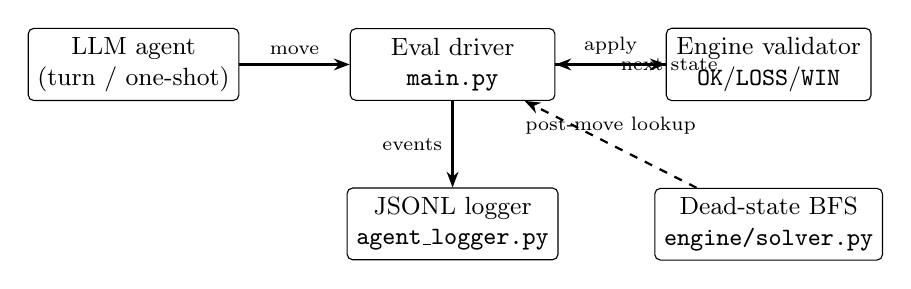
\begin{tikzpicture}[
        node distance=1.1cm and 1.4cm,
        box/.style={draw, rounded corners=2pt, align=center, minimum width=2.6cm,
                    minimum height=0.85cm, font=\small},
        arrow/.style={-{Stealth[length=2mm]}, thick},
    ]
        \node[box] (agent) {LLM agent\\(turn / one-shot)};
        \node[box, right=of agent] (driver) {Eval driver\\\texttt{main.py}};
        \node[box, right=of driver] (validator) {Engine validator\\\texttt{OK}/\texttt{LOSS}/\texttt{WIN}};
        \node[box, below=of validator] (solver) {Dead-state BFS\\\texttt{engine/solver.py}};
        \node[box, below=of driver] (logger) {JSONL logger\\\texttt{agent\_logger.py}};

        \draw[arrow] (agent) -- node[above, font=\scriptsize]{move} (driver);
        \draw[arrow] (driver) -- node[above, font=\scriptsize]{apply} (validator);
        \draw[arrow] (validator) -- node[right, font=\scriptsize]{next state} (driver);
        \draw[arrow] (driver) -- node[left, font=\scriptsize]{events} (logger);
        \draw[arrow, dashed] (solver) -- node[above, font=\scriptsize]{post-move lookup} (driver);
    \end{tikzpicture}
    \caption{HLG system architecture. The main loop consults the agent each turn,
    receives a proposed move, and forwards it to the game engine's validator, which
    returns the next state and an \texttt{OK}/\texttt{LOSS}/\texttt{WIN} status. Logged
    events flow through observability into JSONL traces. Dead-state detection runs as
    an offline BFS pass per level (bottom-right) and is consulted post-move; it does
    \emph{not} live inline in the validator.}
    \label{fig:arch}
\end{figure}

\subsection{Production pipeline}

HLG is small enough that a heavyweight studio model is not warranted. The pipeline is
linear:

\begin{enumerate}[leftmargin=1.5em]
    \item \textbf{Source levels.} 34 \texttt{.txt} grids drawn from
      grahambarrgraham's repository \cite{grahambarrgrahambloxorz}.
    \item \textbf{Parse.} \texttt{engine/state.py} tokenizes each level into a tile
      grid and a switch / teleport wiring table.
    \item \textbf{Verify.} \texttt{verify\_solutions.py} replays a known-optimal
      action sequence per level and asserts the engine reports \texttt{WIN}.
    \item \textbf{Precompute dead states.} \texttt{engine/solver.py} runs forward BFS
      from the initial state, records reverse edges, then runs backward BFS from
      WIN-adjacent states. Reachable states not in the backward closure are dead.
    \item \textbf{LLM harness.} The agent drivers in \texttt{main.py} run the engine
      against a model API, in either turn or one-shot mode, optionally chained via
      sequence mode.
\end{enumerate}

\subsection{Engine}

The engine is dependency-free Python. Three modules:
\begin{itemize}[leftmargin=1.5em]
    \item \texttt{engine/state.py} parses level files and computes the next block
      position given a direction (a pure function of the current orientation).
    \item \texttt{engine/validator.py} applies a move and returns
      \texttt{(status, next\_state)}. It checks boundary, missing-tile, and
      weak-tile-upright conditions; it activates strong, weak, and teleport tiles; and it
      handles split mode (two-target teleports) including the merge logic for
      reuniting the halves.
    \item \texttt{engine/solver.py} computes the per-level dead-state set via
      two-phase BFS.
\end{itemize}

We accurately disclose the following: the validator currently does \emph{not} consult
the dead-state set in-line. A \texttt{TODO} marker at line 42 of
\texttt{engine/validator.py} flags this as future work. The driver in \texttt{main.py}
performs the lookup explicitly after each move and tags the attempt with
\texttt{[DEAD]} rather than \texttt{[LOSS]}. This separation keeps the validator
provably side-effect-free with respect to history-dependent solver caches.

\subsection{Environment design constraints}

\begin{itemize}[leftmargin=1.5em]
    \item \textbf{Mechanic diversity}: the 34 levels collectively exercise plain
      tiles, weak tiles, both switch types, single- and two-target teleports, and split
      mode.
    \item \textbf{Move-count diversity}: optimal solution lengths range from 7 to
      113. Difficulty as measured by optimal length is approximately monotone in
      level index.
    \item \textbf{Verifiable correctness}: every level has a reference solution
      replayed in \texttt{verify\_solutions.py}; corrupting a level breaks CI.
\end{itemize}

\subsection{Automated validation}

The validation pipeline has three layers:
\begin{enumerate}[leftmargin=1.5em]
    \item \emph{Solution replay.} Each level's reference solution is replayed; a
      \texttt{WIN} is required.
    \item \emph{Dead-state computation.} Each level's dead-state set is computed at
      driver startup. The BFS terminates within seconds per level.
    \item \emph{Random-policy probe.} A uniformly random policy is run for $N$ steps
      against every level; non-tutorial levels must not be solvable by chance.
\end{enumerate}

\subsection{Dataset composition}
\label{sec:dataset}

\begin{table}[h]
\centering
\caption{HLG dataset composition. Tutorial level 0 is excluded from official scoring.
Optimal lengths $L_l$ are taken from \texttt{verify\_solutions.py}.}
\label{tab:dataset}
\begin{tabular}{@{}lrrrr@{}}
\toprule
\textbf{Subset} & \textbf{Levels} & \textbf{$N$} & \textbf{$L_l$ range} & \textbf{Notes} \\
\midrule
Tutorial      & 0          & 1  & --            & No mechanics; single open arena. \\
Public Demo   & 1--9       & 9  & 7--34         & No switches before level 8. \\
Semi-Private  & 10--24     & 15 & 33--82        & Used for the official leaderboard. \\
Fully-Private & 25--33     & 9  & 51--128       & Reserved for the HLG Challenge. \\
\midrule
Total         &            & 34 & 7--128        & \\
\bottomrule
\end{tabular}
\end{table}


\begin{figure}[h]
    \centering
    \begin{subfigure}{0.45\linewidth}
        \centering
        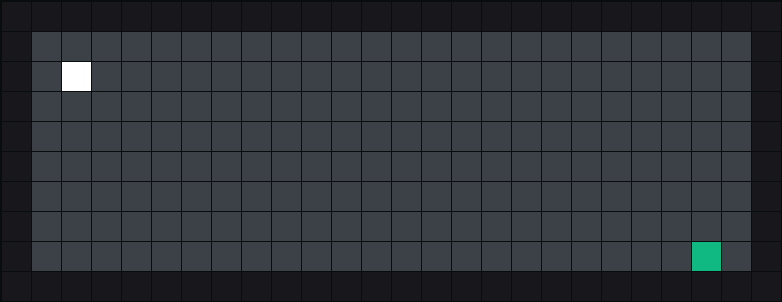
\includegraphics[width=\linewidth]{figures/level0.png}
        \caption{Level 0 — tutorial. No mechanics; the agent only navigates from start (purple) to end (green).}
    \end{subfigure}
    \hfill
    \begin{subfigure}{0.45\linewidth}
        \centering
        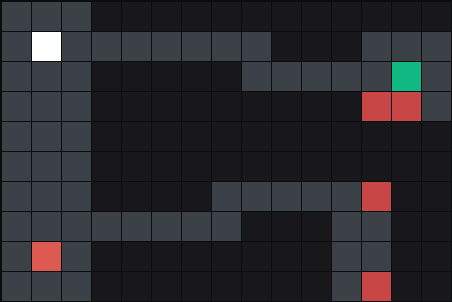
\includegraphics[width=\linewidth]{figures/level17.png}
        \caption{Level 17 — multiple bridge groups and weak tiles. Optimal solution has 104 moves.}
    \end{subfigure}
    \caption{Two levels at the extremes of the difficulty curve. The block (white) starts on the purple start tile and must end UPRIGHT on the green end tile. Red tiles are switches; muted-red tiles are weak.}
    \label{fig:levels}
\end{figure}

\section{Measuring performance on HLG}
\label{sec:measuring}

\subsection{HLG-RHAE}
\label{sec:rhae}

HLG-RHAE is the per-level Relative Human Action Efficiency metric, structurally
identical to ARC-AGI-3's RHAE \cite{arcagi3}. For each level $l$ in $\{1,\ldots,n\}$ with
$n=34$:

\begin{definition}[Per-level efficiency]\label{def:perlevel}
Let $a_l$ be the agent's move count on its first WIN of level $l$ (or $\infty$ if the
level is never won), and let $h_l$ be the human-baseline move count. The per-level
efficiency score is
\begin{equation}
S_l \;=\; \min\!\left(1.15,\ \frac{h_l}{a_l}\right)^2,
\qquad S_l \coloneqq 0 \ \text{if level $l$ unsolved.}
\label{eq:Sl}
\end{equation}
\end{definition}

\begin{definition}[HLG-RHAE]\label{def:rhae}
With linear weights $w_l = l$ and the set of solved levels $\mathcal{W}$,
\begin{equation}
\mathrm{HLG\text{-}RHAE}
\;=\; \min\!\left(
    \frac{\sum_{l\in\mathcal{W}} w_l}{\sum_{l=1}^{n} w_l},\
    \frac{\sum_{l=1}^{n} w_l \cdot S_l}{\sum_{l=1}^{n} w_l}
  \right).
\label{eq:rhae}
\end{equation}
\end{definition}

The first term in the outer $\min$ is a per-environment cap that ties the maximum
achievable score to the weighted fraction of levels solved. This prevents an agent that
solves only the early easy levels from receiving a high score by being slightly
super-efficient on those levels.

\subsection{Design decisions}
\label{sec:scoring-design}

\paragraph{Linear level weighting.} Level $l$ contributes weight $w_l = l$. Because
optimal solution length grows roughly monotonically in level index, this weight schedule
matches difficulty.

\paragraph{Per-level 1.15$\times$ cap.} If an agent finds a 2-action exploit on a
20-action level, an uncapped ratio would produce $10\times$ credit and overwhelm the
environment average. The cap follows ARC's rationale.

\paragraph{Power-law (squared) efficiency term.} A linear term gives 50\% credit at
$2\times$ human baseline; the squared term gives $25\%$. This sharpens the metric's
discrimination between near-human and substantially worse performance.

\paragraph{Action budget of 5$\times$ optimal.} For a level with optimal length $L_l$,
the agent is terminated after $5 L_l$ moves. This keeps API costs bounded and is
identical in spirit to ARC's $5n$ rule applied to the human-baseline median.

\paragraph{First-success only.} Subsequent attempts on an already-won level do not
modify the score. This mirrors a ``first-contact'' interpretation of generalization.

\subsection{Leaderboards}
\label{sec:leaderboards}

We report two leaderboards.

\paragraph{Official.} The official leaderboard uses the canonical system prompt from
\texttt{system\_prompt.md}, no harness, and the \texttt{none}-effort and \texttt{high}-effort
variants of each model. This produces an apples-to-apples comparison across providers.

\paragraph{Community.} The community leaderboard accepts arbitrary harnesses and
self-reported scores, in the spirit of ARC's community track.

% Auto-generated by scripts/build_paper_assets.py.
% Re-run after extract_leaderboard.py to refresh.
\begin{table}[h]
\centering
\caption{Initial frontier-model HLG-RHAE on the full scoring set (levels 1--33), turn mode, parallel runs. Numbers are computed by \texttt{scripts/extract\_leaderboard.py} against the v0.1 baseline ($h_l = L_l$, optimal length). Cost computed at provider-published per-token rates as of March 2026.}
\label{tab:leaderboard}
\small
\begin{tabular}{@{}llrrrrr@{}}
\toprule
\textbf{Provider} & \textbf{Model} & \textbf{Effort} & \textbf{HLG-RHAE} & \textbf{Won} & \textbf{Tokens} & \textbf{Cost (USD)} \\
\midrule
OpenAI & \texttt{oai-gpt-4.1-2025-04-14} & high & 0.18\% & 1/1 & 23,546 & \$0.12 \\
Anthropic & \texttt{claude-opus-4-6} & high & 0.00\% & 0/1 & 0 & \$0.00 \\
\bottomrule
\end{tabular}
\end{table}


\section{Human calibration and solvability}
\label{sec:calibration}

We disclose openly that v0.1 of HLG ships without controlled human-trial data. As
described in Section~\ref{sec:scoring-design}, the v0.1 baseline $h_l$ is taken to be
$L_l$, the optimal solution length verified by \texttt{verify\_solutions.py}. This
introduces two systematic biases that we believe should be visible to readers and
correctable in future versions.

\paragraph{$h_l = L_l$ overstates human efficiency.} Real first-contact human players
are expected to take materially more than $L_l$ actions on hard levels because they
must spend actions exploring the environment before committing to a plan. ARC-AGI-3
reports an optimal-vs-best-first-run gap that is roughly 2--5$\times$ on most levels
\cite{arcagi3}. We therefore expect frontier-model HLG-RHAE scores under v0.1 to be
\emph{lower} than they will appear under v0.2 with real human baselines.

\paragraph{Optimal solutions are pinned to a single trajectory.} The reference solutions
in \texttt{verify\_solutions.py} are not necessarily unique. For levels with multiple
optimal trajectories we use the first one found by the breadth-first solver. This is
consequence-free for the metric (the move count is what matters), but downstream
analyses that examine \emph{which} actions the agent takes should not assume the
reference solution is the only optimal choice.

\subsection{Planned testing protocol for v0.2}

We plan to run a small-scale Prolific study with the following protocol, modeled on the
ARC-AGI-3 testing protocol:

\begin{itemize}[leftmargin=1.5em]
    \item 10 participants per level. Each participant is exposed to each level for the
      first time.
    \item No level-specific instruction. The system prompt that LLMs receive is
      summarized into a one-page interactive tutorial covering only the rules.
    \item Soft cutoff of 20 minutes per level; hard cutoff of 30 minutes.
    \item Participants may reset a level but cannot revisit a previously completed
      level.
    \item The human baseline $h_l$ is defined as the upper-median of the action counts
      among completers on level $l$.
\end{itemize}

\subsection{Initial level-difficulty signal}

In the absence of human data we use $L_l$ as the difficulty signal. Across the 34
levels, $L_l \in [7, 113]$ with median 35 and the curve is approximately monotone in
level index past the tutorial (level 0).

\section{Initial frontier-model evaluations}
\label{sec:evals}

We evaluate twelve model configurations against HLG, drawn from the model list in
\texttt{model\_list.txt}. Six base models, each at \texttt{none} and \texttt{high}
reasoning effort:

\begin{itemize}[leftmargin=1.5em]
    \item \texttt{claude-sonnet-4-6}
    \item \texttt{claude-opus-4-6}
    \item \texttt{gpt-5.4}
    \item \texttt{gpt-5.4-nano}
    \item \texttt{oai-gpt-5-2-2025-12-11}
    \item \texttt{oai-gpt-4.1-2025-04-14}
\end{itemize}

\subsection{Evaluation regimes}

For each model we report results in three regimes:
\begin{enumerate}[leftmargin=1.5em]
    \item \textbf{Turn (parallel).} 34 levels run in parallel, each level with an
      isolated session and accumulating conversation history within attempts.
    \item \textbf{Turn (sequence).} 34 levels run sequentially with prior level
      attempts injected into the next level's first user message via
      \texttt{<level\_history>}.
    \item \textbf{One-shot.} The model emits a full move sequence per attempt; no
      intermediate observations are provided.
\end{enumerate}

\subsection{Results}

Per-model HLG-RHAE values, level-completion counts, and total token usage are reported in
Table~\ref{tab:leaderboard} (in Section~\ref{sec:measuring}). Figure~\ref{fig:perf}
visualizes the cost--RHAE Pareto frontier across configurations.

\begin{figure}[t]
    \centering
    % Auto-generated by scripts/build_paper_assets.py
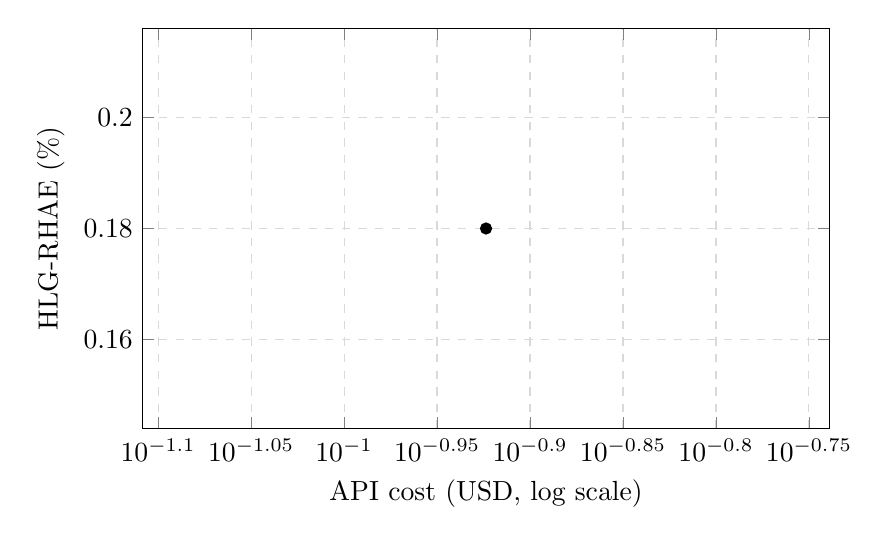
\begin{tikzpicture}
\begin{axis}[
    width=0.85\linewidth, height=0.55\linewidth,
    xmode=log,
    xlabel={API cost (USD, log scale)},
    ylabel={HLG-RHAE (\%)},
    grid=both,
    grid style={dashed, gray!30},
    only marks,
    nodes near coords,
    nodes near coords align={above},
    point meta=explicit symbolic,
]
\addplot[mark=*, mark size=2pt] coordinates {
        (0.1192, 0.1800)
};
\end{axis}
\end{tikzpicture}

    \caption{HLG-RHAE versus dollar cost across the evaluated configurations (turn
    mode, official leaderboard). Each point is a (model, reasoning-effort) pair.
    Dollar cost is computed from per-token rates published by each provider as of
    March 2026 (see \texttt{scripts/build\_paper\_assets.py} for the rate table). The
    pgfplots source is auto-generated from \texttt{data/leaderboard.json}; rerun
    \texttt{python scripts/build\_paper\_assets.py} to refresh.}
    \label{fig:perf}
\end{figure}

\subsection{Qualitative findings}

\paragraph{Loss vs.\ dead state.} Across configurations, frontier models routinely fail
to distinguish a legal-but-unwinnable state from an illegal move. They activate a
\texttt{close} switch that closes the only required bridge, then continue planning as
if the future were unconstrained. Models receive an explicit \texttt{[DEAD]} tag in
their next-attempt context; this often is not enough to identify the earlier branching
point that caused the dead end.

\paragraph{Weak-tile orientation.} Models often correctly avoid \emph{landing} upright
on a weak tile, but fail to plan a flat traversal of a weak-tile corridor when an
upright landing would otherwise be the most direct path.

\paragraph{Split mode.} Two-target teleport levels separate two halves of the block.
Frontier models in our evaluation rarely succeed on these levels, often outputting the
\texttt{s} action outside of split mode (which is a no-op) or failing to plan for the
merge geometry.

\paragraph{One-shot vs turn.} One-shot mode is materially cheaper but its WIN rate
is uniformly lower than turn mode at matched compute. The gap is largest on levels
with bridge-group toggling, where online correction in turn mode lets the model
recover from a misjudged switch order.

\section{HLG Challenge 2026}
\label{sec:challenge}

We plan to host an HLG Challenge in late 2026, modeled on the ARC Prize annual
competition format. The challenge will run on the fully-private level set (levels 25--33)
plus newly authored levels added in v0.2. Submitted agents will be evaluated against
the same canonical system prompt and the same action / token / wall-clock budgets as the
official leaderboard.

The grand prize threshold is set at 85\% HLG-RHAE on the fully-private set, matching the
ARC-AGI-3 threshold convention. As of v0.1 release no system has cleared 10\% on the
semi-private set; the threshold therefore represents a substantial extrapolation
beyond the present capability frontier.

Specific competition rules, prize amounts, and submission deadlines will be published
on the public leaderboard page (\texttt{/leaderboard} in the docs site) closer to
the event.

\section{Conclusions}
\label{sec:conclusions}

HLG provides a small, fully-verifiable agentic benchmark that exercises long-horizon
planning, irreversible side-effect modeling, and dead-end avoidance on a discrete
spatial domain that frontier LLMs have not been heavily trained on. The benchmark is
deliberately compact (34 levels, ~150 lines of public Python SDK, one engine module per
concern), to make it tractable for independent re-implementation and to keep the
evaluation cost low enough to run as a regression test on every new model release.

Three open problems stand out:

\begin{itemize}[leftmargin=1.5em]
    \item \textbf{Dead-state reasoning.} Models do not yet appear to distinguish
      \texttt{[LOSS]} from \texttt{[DEAD]} in their reasoning chains. Eliciting that
      distinction may require explicit backward-reachability heuristics in the system
      prompt, or training signals that reward identifying the earlier branch point in a
      dead-attempt trajectory.
    \item \textbf{Weak-tile orientation reasoning.} The interaction between block
      orientation and tile fragility is conceptually simple but operationally subtle;
      it is a microcosm of physical-affordance reasoning, and current models struggle
      with it.
    \item \textbf{Split-mode merge planning.} Split mode requires planning over two
      independently controlled bodies that must be reunited; the merge condition
      depends on adjacency at the time of merge. This is the closest HLG approximation
      to multi-agent coordination over shared state.
\end{itemize}

We anticipate v0.2 of HLG will add controlled human trials, a public REST surface
implementing \texttt{hlg-openapi.yaml}, provider adapters under \texttt{hlg.providers},
and an expanded private level set.

\section*{Acknowledgments}
\label{sec:acks}
\addcontentsline{toc}{section}{Acknowledgments}

We thank Damien Clarke, the original author of Bloxorz, for designing the puzzle
mechanics that make this benchmark possible. We thank grahambarrgraham
\cite{grahambarrgrahambloxorz} for assembling and openly publishing the level set, and
tkoz0 \cite{tkoz0bloxorzsolver} for the original BFS solver whose move-encoding
conventions our verifier inherits.

Any modifications to the original level set were made strictly for integration into
this benchmark; full credit for level design and original game mechanics remains with
the respective authors.


\bibliographystyle{plainnat}
\bibliography{references}

\end{document}
